% Note : this document use minted package for code listings :
% minted depends on pygments, install using apt package manager
% use -shell-escape to compile
% if errors occur remove _minted-* directory
\documentclass[a4paper]{article}
\usepackage{style}

\usepackage[newfloat]{minted} %the newfloat option places caption on top of listings
\definecolor{bg}{rgb}{0.95,0.95,0.95} %code background color

\title{
  \bfseries AWS Machine Learning Engineer Nanodegree \\
  Capstone Project \\
  Arvato Customer Acquisition Prediction Using Supervised Learning
}
\author{Fady Morris Milad\thanks{Email: \href{mailto:fadymorris86@gmail.com}{fadymorris86@gmail.com}}}


\usepackage{pgf}
\usepackage{lmodern}

\begin{document}
\pagenumbering{roman}

\pretitle{%from package titling
  \begin{center}
    \LARGE
    
\includegraphics[width=0.75\textwidth]{udacity-logo}\\[\bigskipamount]
  }

  \date{February 22, 2022} %\date{\today}

  {
    \makeatletter
    \addtocounter{footnote}{1} % to get dagger instead of star
    \renewcommand\thefootnote{\@fnsymbol\c@footnote}%
    \makeatother
    \maketitle
  }
  \newpage
  \tableofcontents
  \newpage

  \pagenumbering{arabic}
  \section{Definition}
  \subsection{Project Overview}

  {
    % \color{red}
    % \begin{figure}[H]
    %   \centering
    %   \caption{Frequency of unknown values representation in metadata}
    %   \includegraphics{test}
    % \end{figure}


    % \begin{figure}[H]
    %   \centering
    %   \caption{Test Figure 500}
    %   \label{fig:test}
    %   \input{../output/figures/test.pgf}
    % \end{figure}
    % }

    \lettrine[lines=3,findent=2pt, lraise=0.2]{\fbox{\textbf{A}}}{rvato} is a company that provides financial services, IT services, and supply chain management services solutions to other businesses. It has a large base of global customers. Its solutions focus on automation and data analytics.\cite{arvato-company}

    Arvato's customer base comes from a wide variety of businesses, such as insurance companies, telecommunications, media education, and e-commerce. 

    Arvato analytics is helping businesses to take important decisions and gain insights from data. It uses data science and machine learning to meet business goals and gain customer satisfaction.

    Arvato is owned by Bertelsmann \cite{bertelsmann-company}, which is a media, services, and education company that operates in about 50 countries around the world.

    In this project, Arvato is helping a mail-order company that sells organic products in Germany to build a model to predict which individuals are most likely to convert into becoming customers for the company by analyzing marketing campaign mailout data.

    Customer retention and churn were addressed in the following academic research papers: 
    \parencite{al-shatnwai_predicting_2020} and \cite{zhuang_research_2018}

    We have a proprietary dataset that contains 42,982 training samples and 42,833 testing samples. Both the datasets have 366 features and the testing set doesn't have the label column.

    We will use Amazon SageMaker to train a machine learning model using the training set, and then generate predictions using the testing set. We will validate the generated predictions using \href{https://www.kaggle.com/docs/api}{Kaggle API} which has a \href{https://www.kaggle.com/c/udacity-arvato-identify-customers}{dedicated competition} for this problem.


    \subsection{Problem Statement}

    The problem can be stated as: ``Given the existing marketing campaign demographic data of customers who responded to marketing mails, how can we predict whether a new person will be a potential customer for the mail-order company?''

    Here we use \emph{XGBoost}, which is a supervised learning algorithm,  and train a model that will help the company make such predictions and decide whether is a person is a potential candidate to be a customer for the company or not.

    \subsection{Metrics}
    \label{sec:metrics}
    Our problem is a binary classification problem. Our classes are labeled either 0 (the individual is not a customer) or 1 (the individual became a customer), and the dataset is imbalanced as shown in \autoref{tab:label-counts-freqs} - \nameref{tab:label-counts-freqs}.

    To measure how close our predictions to the ground truth labels, we will use two classification metrics: \emph{ROC-AUC score} and \emph{log-loss score}.

    \subsubsection{ROC-AUC Score}
    \label{sec:accuracy}
    \emph{ROC-AUC} stands for the \textbf{R}eceiver \textbf{O}perating \textbf{C}haracteristic \textbf{A}rea \textbf{U}nder \textbf{C}urve. This is the metric used by the Kaggle Competition to evaluate the test data.

    The receiver operator characteristic (ROC) curve is a plot of the \emph{true positive rate}(TPR) against the \emph{false positive rate} at various threshold values.

    The area under ROC curve is a metric that measures the ability of the classifier to distinguish between positive and negative classes.

    \subsubsection*{ROC-AUC Metric interpretation:}

    \begin{itemize}
    \item \textbf{AUC = 1}: The classifier perfectly separates the positive and the negative classes.
    \item \textbf{0.5 < AUC < 1}: The classifier can distinguish between negative and positive classes with a high probability. The higher is better.
    \item \textbf{AUC = 0.5}: is not different from a random guess. The classifier is unable to distinguish between classes.
    \item \textbf{AUC = 0}: The classifier predicts all negatives as positives and vice versa.
    \end{itemize}

    \subsubsection{Log-Loss}
    \label{sec:log-loss}
    Log-loss is a metric that indicates how close the prediction probability is to the corresponding actual value (0 or 1 in our case). The more the predicted probability diverges from the actual value, the higher is the log-loss value.

    {
      The log-loss function $\mathcal{L}$ can be defined by the following equation:
      
      \newcommand{\yi}{y^{(i)}}
      \newcommand{\probi}{p^{(i)}}

      $$
      \mathcal{L}\left(\probi, \yi\right)
      = \frac{1}{m} \sum_{i=1}^m \left[\yi\log\left(\probi\right)
        + \left(1 - \yi\right) \log\left(1-\probi\right)
      \right]
      $$


      \textbf{Where:}

      $\yi$: The actual (ground truth) label for the $i^{\text{th}}$ training example.

      $\probi$: The predicted probability of class 1 for the $i^{\text{th}}$ training example.
      
    }

    In our project, the log-loss objective metric is used by Amazon SageMaker hyperparameter tuning to find the best combination of hyperparameters that minimize the loss function.


    \section{Analysis}
    \subsection{Data Exploration}
    \label{sec:data-exploration}

    The dataset is a private dataset. It is used with permission from Arvato for use in the nanodegree project.

    \subsubsection{Raw Dataset Files}
    \label{sec:raw-dataset-files}


    There are two files of the dataset that we are concerned with:
    \begin{itemize}
    \item \texttt{Udacity\_MAILOUT\_052018\_TRAIN.csv}: Demographic data for people in Germany that were targeted by the marketing mailing campaign. It contains data for 42,982 individuals.

      This training dataset has 367 columns, 366 of them are demographic features, and one label column \code{['RESPONSE']}
    \item \texttt{Udacity\_MAILOUT\_052018\_TEST.csv}: The testing dataset, contains data for 42,833 individuals and it has 366 columns of the demographic features, this dataset has no label columns and will be tested using Kaggle API for \href{https://www.kaggle.com/c/udacity-arvato-identify-customers/data}{Udacity+Arvato: Identify Customer Segments} competition.
    \end{itemize}

     Two metadata files that contain a data dictionary for the demographic features in the previous dataset files.

    \begin{itemize}
    \item \texttt{DIAS Information Levels - Attributes 2017.xlsx}: An excel sheet that contains a top-level organization of demographic features, their description, and some notes.
    \item \texttt{DIAS Attributes - Values 2017.xlsx}: An excel sheet that contains demographic features sorted alphabetically, their description, their values, and the meaning of each value.
    \end{itemize}
\pagebreak
    \subsubsection{The Dataset Metadata}
    \label{sec:dataset-metadata}

    The dataset metadata is described in \texttt{DIAS Attributes - Values 2017.xlsx} 

    \begin{itemize}
    \item It has the following columns :
      
      \begin{tabular}[H]{l l}
        \code{'attribute'}& Name of the dataset feature.\\
        \code{'description'}& Description of the dataset feature (corresponding to \code{'attribute'}.\\
        \code{'value'}& Contains a valid range of values for each attribute.\\
        \code{'meaning'}& Meaning of each value of the values (corresponding to \code{'value'}). 
      \end{tabular}
    \item The metadata file has 314 feature entries, while the training dataset contains 365 features, so, there is a mismatch between some of the dataset features and their metadata entries and we have to examine and correct them manually.
    \item For the \code{'value'} column, some entries are invalid or contain multiple entries. Example: \code{"-1, 9"}, \code{"-1, 0"}, and \code{"..."}.
    \item After metadata cleaning, it is noted that some codes represent \emph{unknown values}. They are summarized in \autoref{tab:unknown-freqs} and plotted in \autoref{fig:dataset-hbar}
      
      \begin{table}[H]
\centering
\caption{Frequency counts of unknown value numeric codes}
\label{tab:unknown-freqs}
\begin{tabular}{rr}
\toprule
code & frequency \\
\midrule
-1 & 230 \\
9 & 75 \\
0 & 66 \\
10 & 12 \\
\bottomrule
\end{tabular}
\end{table}


    \end{itemize}


    \subsubsection{The Training Dataset}
    \label{sec:training-dataset}

    The raw training dataset is in the file \texttt{Udacity\_MAILOUT\_052018\_TRAIN.csv}.

    A quick examination of the dataset showed that the dataset is highly skewed (imbalanced). only 1.24\% of the individuals targeted by the marketing campaign would respond to it as shown in \autoref{tab:label-counts-freqs}:

    \begin{table}[H]
\centering
\caption{Label Counts and Frequencies}
\label{tab:label-counts-freqs}
\begin{tabular}{rrr}
\toprule
response & count & percentage \\
\midrule
0 & 42,430 & 98.76 \% \\
1 & 532 & 1.24 \% \\
\bottomrule
\end{tabular}
\end{table}



    After cleaning the dataset, the features were categorized into numeric, nominal, and ordinal. The features are also divided into two subsets: features that have metadata and extra features that don't have metadata.

    \autoref{tab:dataset-feature-types} shows the distribution of feature types. And a plot is shown in \autoref{fig:feature-types}.
    \begin{table}[H]
\centering
\caption{Dataset feature types}
\label{tab:dataset-feature-types}
\begin{tabular}{llr}
\toprule
type & subset & frequency \\
\midrule
nominal & extra & 39 \\
nominal & metadata & 64 \\
numeric & extra & 9 \\
numeric & metadata & 7 \\
ordinal & extra & 8 \\
ordinal & metadata & 238 \\
\bottomrule
\end{tabular}
\end{table}



    There are many problems with this dataset:
    \begin{itemize}
    \item After exploratory data analysis, it was found that the training dataset has 56 columns that don't have metadata and should be categorized and examined manually.
    \item Some columns have mixed data types, for example the featrues \code{['CAMEO_DEUG_2015', 'CAMEO_INTL_2015']} have the invalid values \code{['X', 'XX']}.
    \item Some dataset columns have different names than their corresponding metadata entries (for example: \code{'D19_.*'} columns). They should be renamed to match the metadata. The metadata will be used later in the \nameref{sec:data-preprocessing} subsection to check for the valid range of values of every dataset feature.
    \item 67 features have more than 30\% missing values. (See \autoref{fig:missing-values})
    \item 98 features are highly correlated with other features in the dataset, with a Pearson's $r$ correlation coefficient greater than $0.6$. A heatmap of highly correlated features is shown in \autoref{fig:correlation-heatmap}.
    \item 13.41\% of training samples are duplicates. (See \autoref{fig:duplicate-percent}).
    \item Numerical features have outliers that are more than three standard deviations away from the mean. The percentages of outliers for every numeric feature are shown in \autoref{tab:outlier-percent} and \autoref{fig:outliers-numeric}.
      
      \begin{table}[H]
\centering
\caption{Percentage of outliers for each numerical feature}
\label{tab:outlier-percent}
\begin{tabular}{lr}
\toprule
feature & percentage of outliers \\
\midrule
ANZ\_HAUSHALTE\_AKTIV & 6.81\% \\
ANZ\_HH\_TITEL & 7.20\% \\
ANZ\_PERSONEN & 3.88\% \\
ANZ\_TITEL & 4.11\% \\
EINGEFUEGT\_AM & 9.38\% \\
EINGEZOGENAM\_HH\_JAHR & 3.34\% \\
GEBURTSJAHR & 0.00\% \\
KBA13\_ANZAHL\_PKW & 7.25\% \\
VERDICHTUNGSRAUM & 9.27\% \\
\bottomrule
\end{tabular}
\end{table}

    \end{itemize}

    \pagebreak
    \subsection{Exploratory Visualization}
    \label{sec:expl-visu}


    \begin{figure}[H]
      \centering
      \caption{Dataset Feature Types}
      \label{fig:feature-types}
      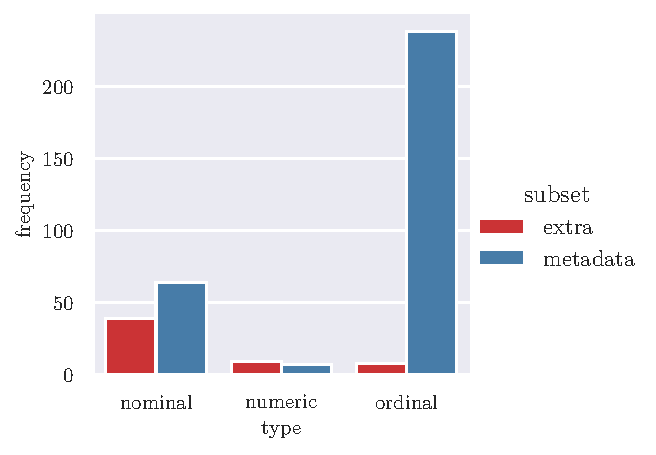
\includegraphics{07_feature-types}
    \end{figure}
    \begin{figure}[H]
      \centering
      \caption{Frequency of unknown values representation in metadata}
      \label{fig:dataset-hbar}
      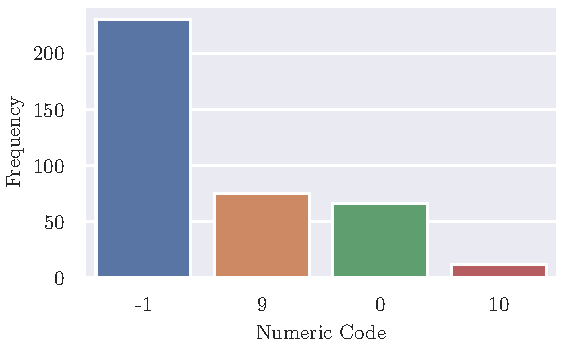
\includegraphics{01_eda_unknown-freqs}
    \end{figure}
    \begin{figure}[H]
      \centering
      \caption{Percentage of duplicate samples.}
      \label{fig:duplicate-percent}
      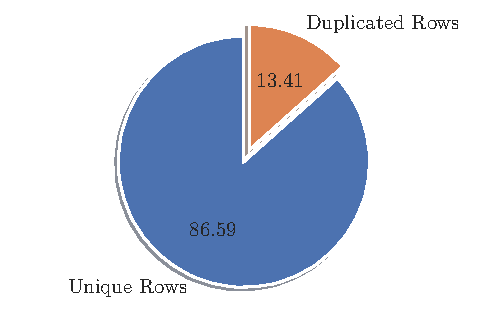
\includegraphics{05_eda_missing-rows}
    \end{figure}
    \begin{figure}[H]
      \centering
      \caption{Features that have more than 30\% of missing values}
      \label{fig:missing-values}
      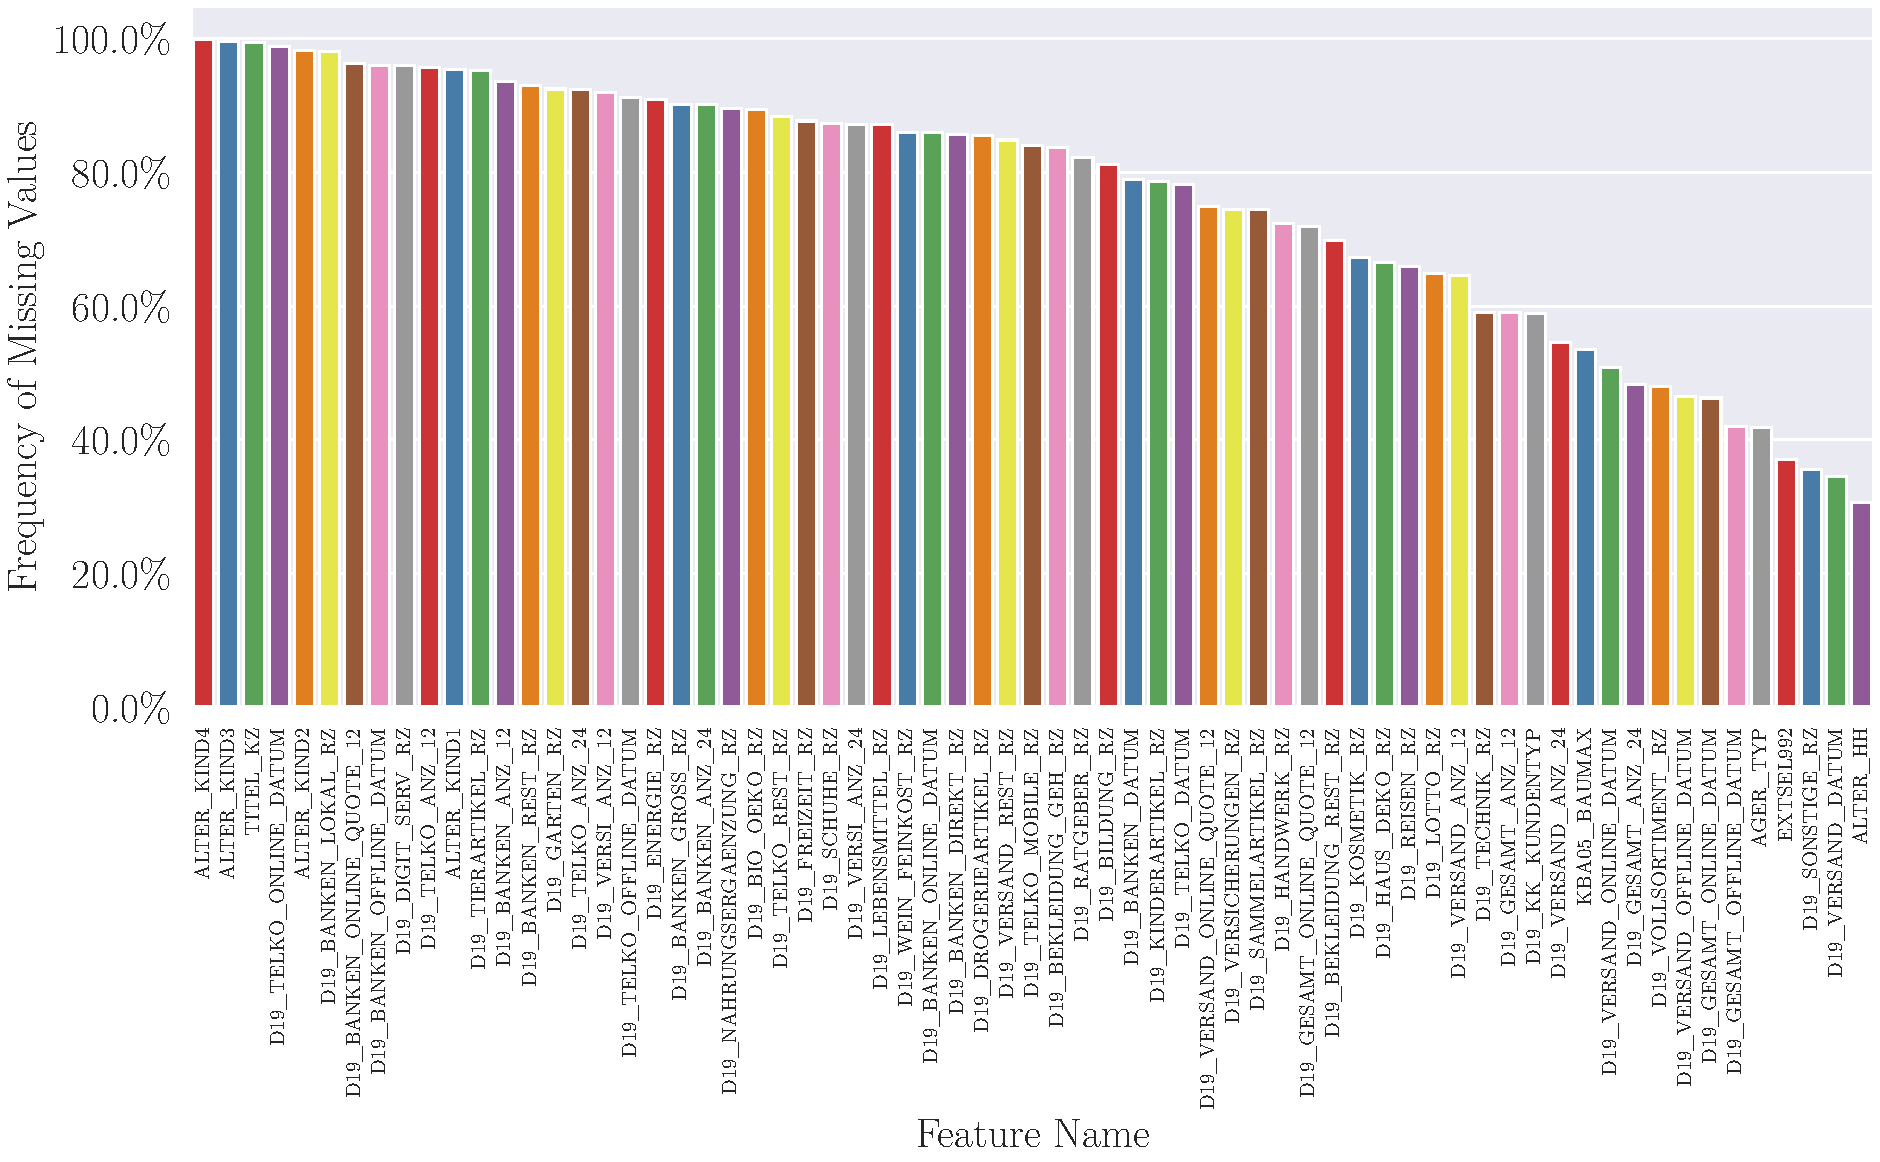
\includegraphics[scale=0.42]{03_missing-values.pdf}
    \end{figure}
    \begin{figure}[H]
      \centering
      \caption{A heat map of highly correlated feature (> 0.75)}
      \label{fig:correlation-heatmap}
      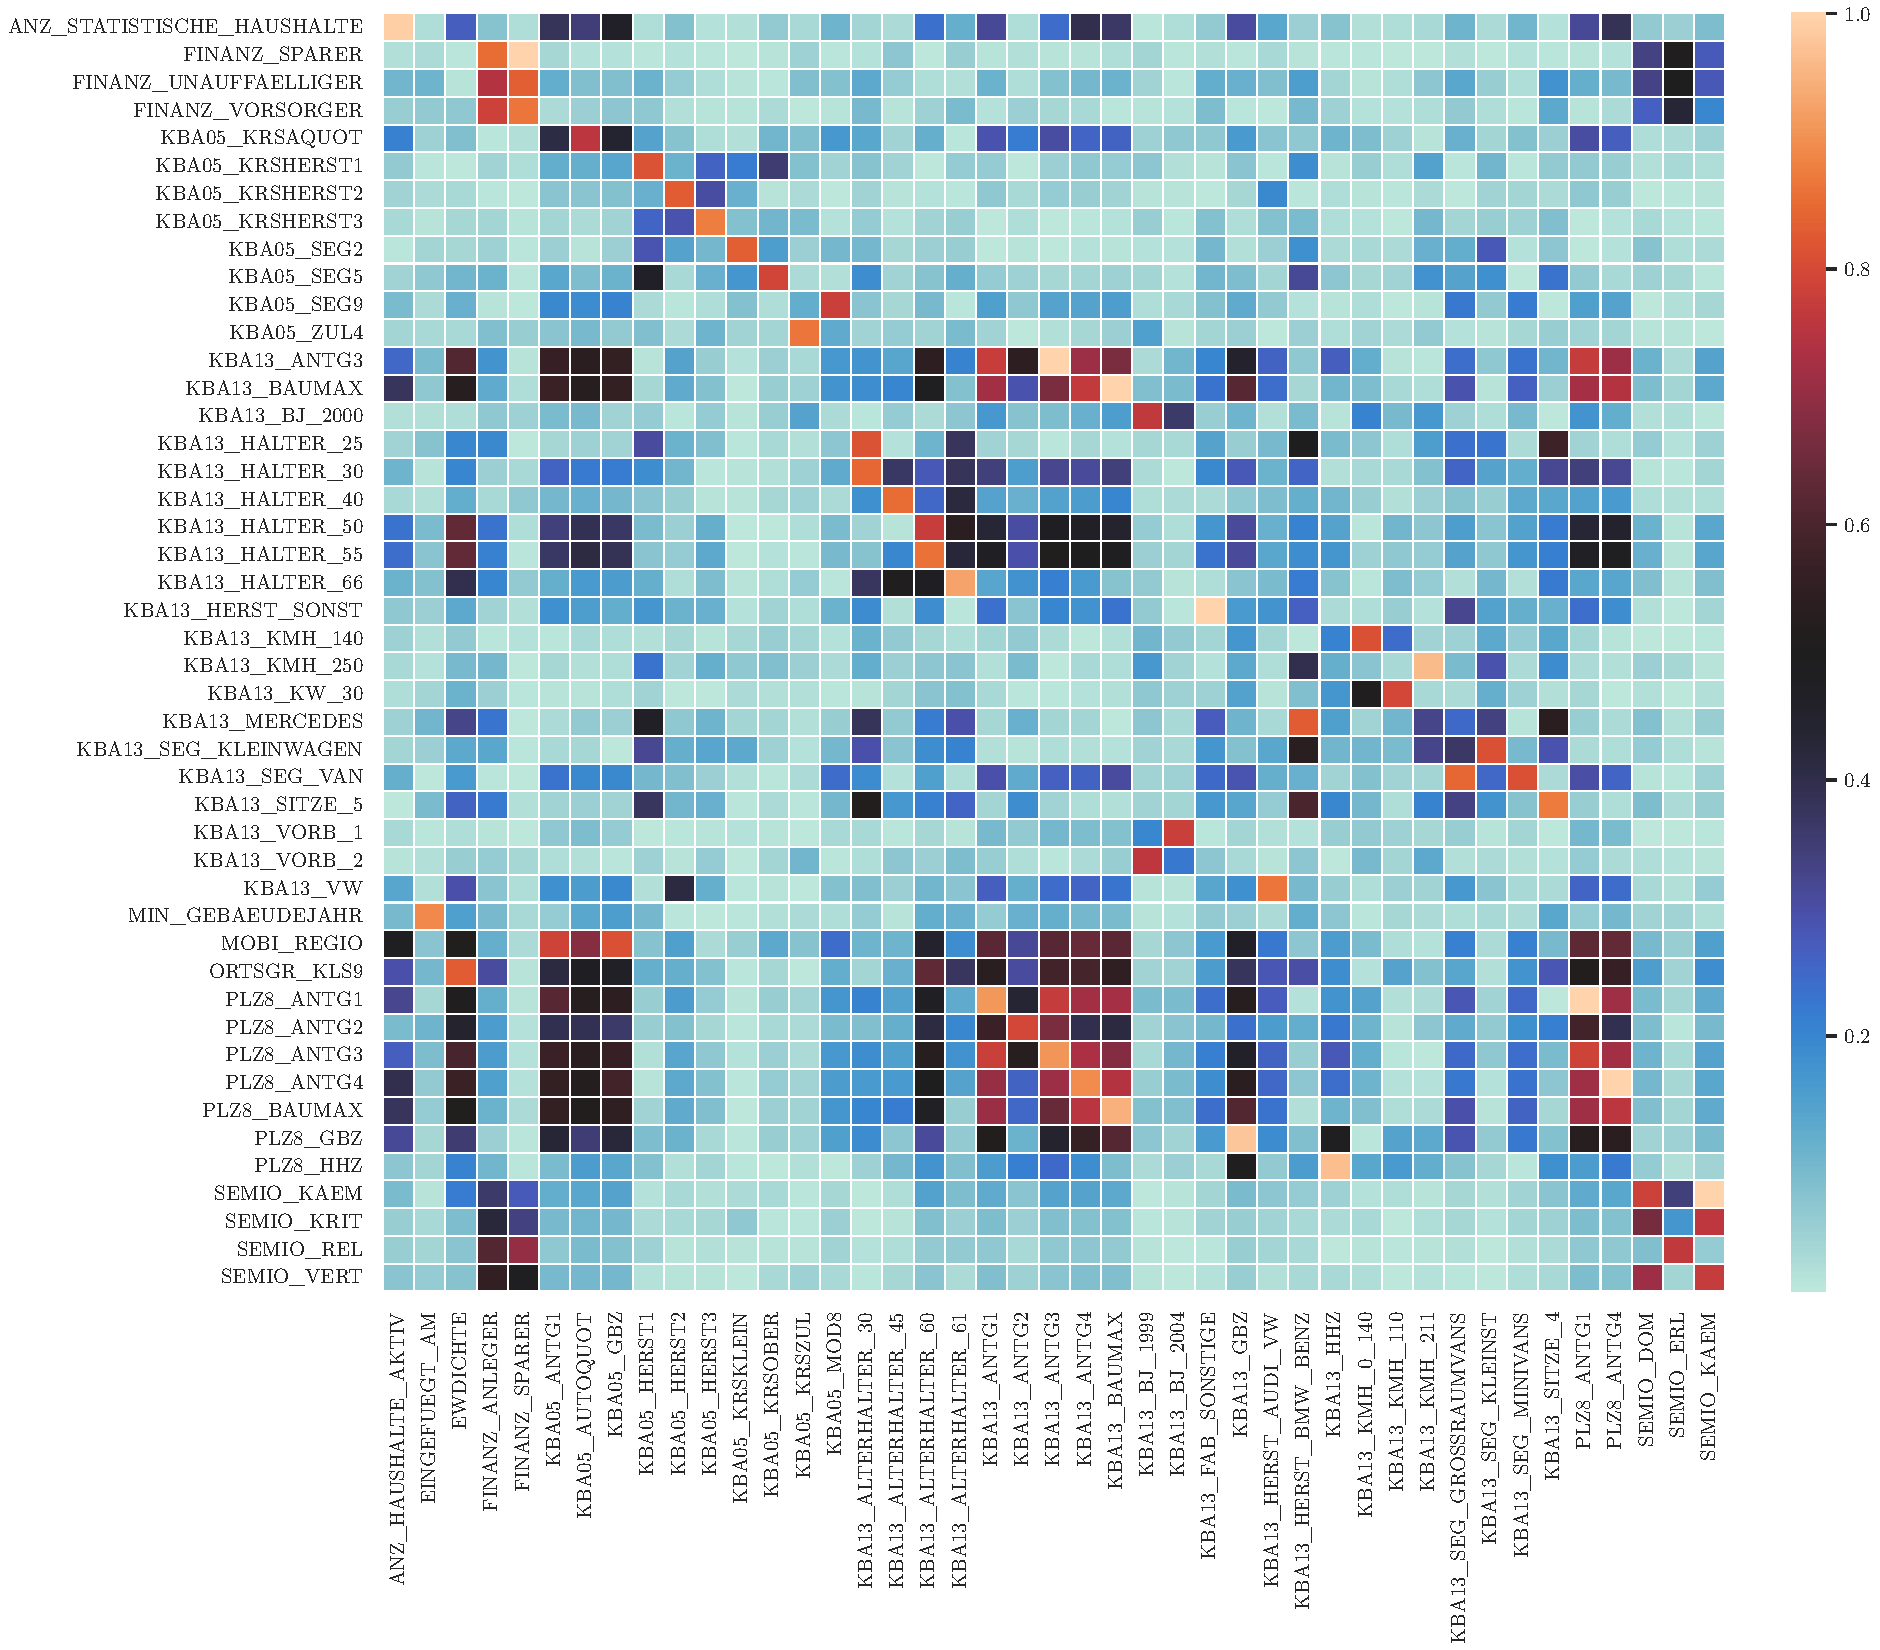
\includegraphics[scale=0.5]{04_correlation-heatmap}
    \end{figure}
    \begin{figure}[H]
      \centering
      \caption{Outliers in numeric values}
      \label{fig:outliers-numeric}
      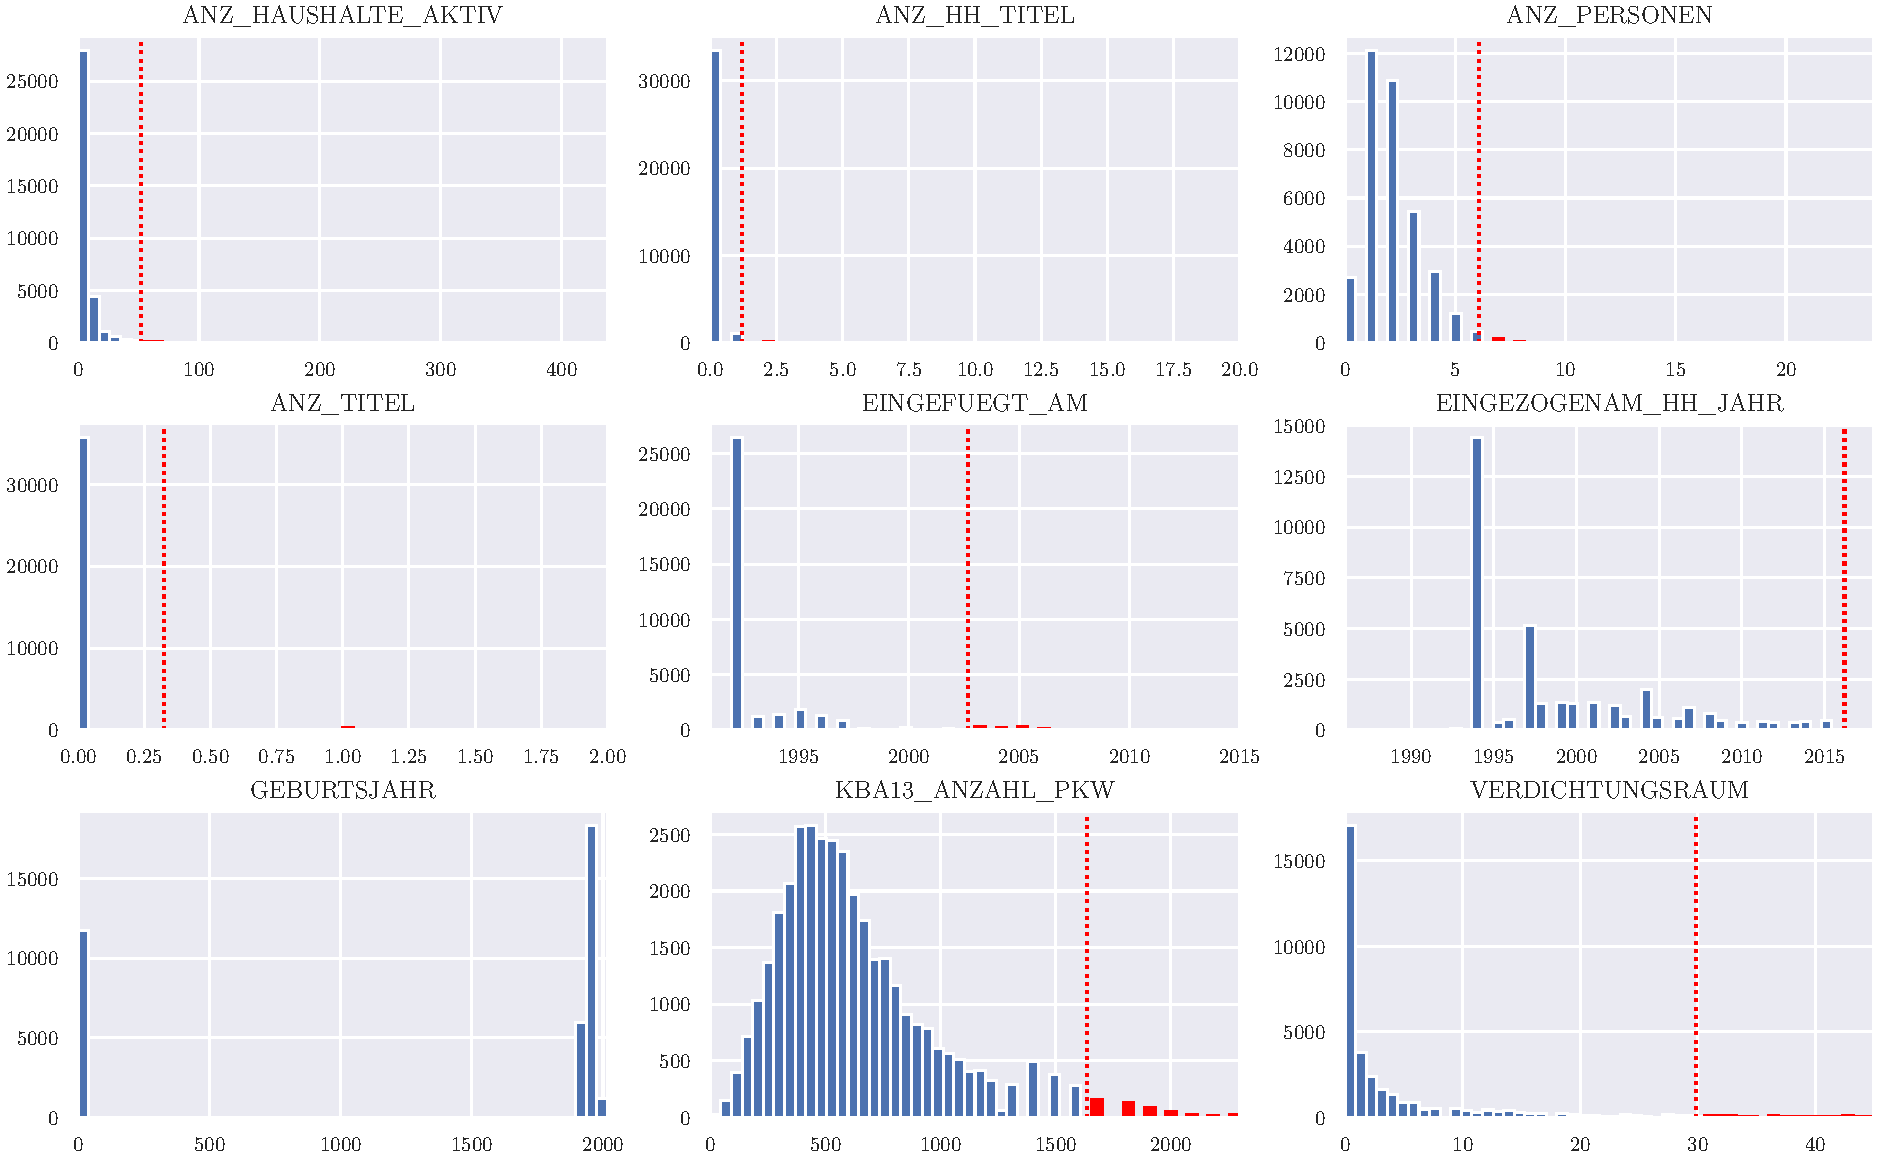
\includegraphics[scale=1]{06_eda_outliers}
    \end{figure}


    \subsection{Algorithms and Techniques}
    Our problem is a binary classification problem. We will use the \href{https://xgboost.readthedocs.io/}{XGBoost} supervised learning algorithm  \cite{friedman_greedy_2000} to predict whether a targeted individual will be a customer (class 1) or not (class 0).

    \emph{XGBoost} stands for e\textbf{X}treme \textbf{G}radient \textbf{Boost}ing. It can be used in supervised learning problems like ours and it is built on the concept of decision tree ensembles. A tree ensemble model is a collection of classification and regression trees (CART) that are called \emph{weak learners}. When (CART) trees are combined their predictive power is enhanced and we obtain a \emph{strong learner}.

    The algorithm has many hyperparameters, but we will only tune the following hyperparameters in \autoref{tab:xgboost-hyperparameters-tunable} using Amazon SageMaker hyperparameter tuning jobs:

    \begin{table}[H]
      \caption{XGBoost Tunable Hyperparameters}
      \label{tab:xgboost-hyperparameters-tunable}
      \centering
      \begin{tabular}{lp{0.7\textwidth}}
        \toprule
        Parameter Name & Description \\
        \midrule
        \code{'num_round'} & The number of rounds to run the training.\\
        \code{'alpha'} & L1 regularization term on weights. Increasing this value makes models more conservative.\\
        \code{'colsample_bylevel'} & Subsample ratio of columns for each split, in each level.\\
        \code{'colsample_bynode'} & Subsample ratio of columns from each node.\\
        \code{'colsample_bytree'} & Subsample ratio of columns when constructing each tree.\\
        \code{'eta'} & Step size shrinkage used in updates to prevent overfitting. After each boosting step, you can directly get the weights of new features. The eta parameter actually shrinks the feature weights to make the boosting process more conservative.\\
        \code{'gamma'} & Minimum loss reduction required to make a further partition on a leaf node of the tree. The larger, the more conservative the algorithm is.\\
        \code{'lambda'} & L2 regularization term on weights. Increasing this value makes models more conservative.\\
        \code{'max_delta_step'} & Maximum delta step allowed for each tree's weight estimation. When a positive integer is used, it helps make the update more conservative. The preferred option is to use it in logistic regression. Set it to 1-10 to help control the update.\\
        \code{'max_depth'} & Maximum depth of a tree. Increasing this value makes the model more complex and likely to be overfit. 0 indicates no limit. A limit is required when \code{'grow_policy'}=depth-wise.\\
        \code{'min_child_weight'} & Minimum sum of instance weight (hessian) needed in a child. If the tree partition step results in a leaf node with the sum of instance weight less than \code{'min_child_weight'}, the building process gives up further partitioning. In linear regression models, this simply corresponds to a minimum number of instances needed in each node. The larger the algorithm, the more conservative it is.\\
        \code{'subsample'} & Subsample ratio of the training instance. Setting it to 0.5 means that XGBoost randomly collects half of the data instances to grow trees. This prevents overfitting.\\        \bottomrule
      \end{tabular}      
    \end{table}
    \vspace{2ex}

    The hyperparameters that have the greatest effect on optimizing the XGBoost evaluation metrics are: \code{'alpha'}, \code{'min_child_weight'}, \code{'subsample'}, \code{'eta'},and \code{'num_round'}.

    The full list of hyperparameters can be found in \href{https://docs.aws.amazon.com/sagemaker/latest/dg/xgboost_hyperparameters.html}{Amazon SageMaker documentation}.

    We will use the \code{'validation:logloss'} evaluation metric described in \autoref{sec:metrics} as our objective function is \code{'binary:logistic'}

    \subsection{Benchmark}
    Our benchmark model is  a simple scikit-learn \href{https://scikit-learn.org/stable/modules/generated/sklearn.linear_model.LogisticRegression.html}{logistic regression} model trained using the default hyperparameters.

    The model was trained using the \emph{train set},  used for inference on the \emph{test set} to generate probabilities, and the resulting probabilities were submitted to Kaggle \href{https://www.kaggle.com/c/udacity-arvato-identify-customers/data}{Udacity+Arvato: Identify Customer Segments} competition for evaluation.

    The resulting AUC-ROC private test score is \textbf{0.71265} as shown in \autoref{fig:benchmark-score}

    \begin{figure}[H]
      \centering
      \caption{Benchmark Model Score}
      \label{fig:benchmark-score}
      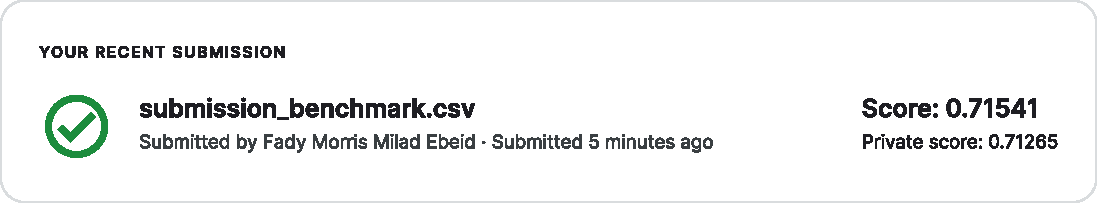
\includegraphics[scale=0.8]{kaggle-score-benchmark}
    \end{figure}


    In \autoref{sec:justification}, the score of our \emph{XGBoost} model will be compared to the score of this baseline model in terms of performance.
    \section{Methodology}

    \subsection{Data Preprocessing}
    \label{sec:data-preprocessing}

    \begin{figure}[H]
      \centering
      \caption{Data Processing Pipeline}
      \label{fig:pipeline}
      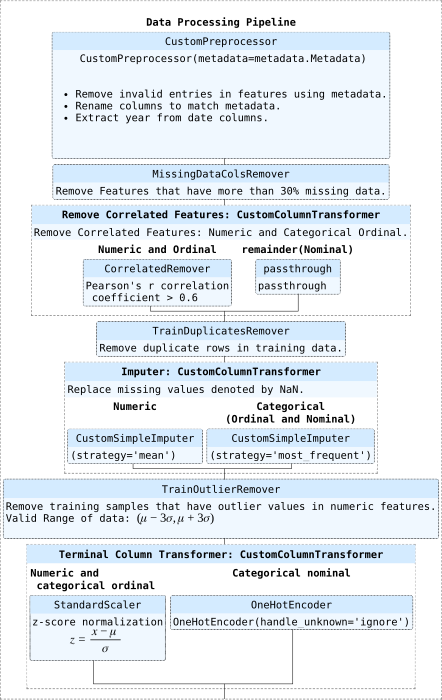
\includegraphics[scale=0.85]{pipeline}
    \end{figure}

    
    The data processing pipeline sketched in \autoref{fig:pipeline} is divided into the following steps:

    \begin{enumerate}
    \item \code{CustomPreprocessor}: a custom preprocessing class that performs the following:
      \begin{itemize}

      \item Fixes the columns that have mixed data types \code{['CAMEO_DEUG_2015', 'CAMEO_INTL_2015']} by replacing the invalid values \code{['X', 'XX']} by \code{NaN}

      \item Drops the \code{['LNR']} column as it is an index column.

      \item Renames all the columns that differ in name between the dataset and the metadata either by regular expressions (For example \code{'D19_.*'} columns) or manually using a dictionary to match the metadata.
        
      \item For categorical (ordinal and nominal) features that have metadata, it checks their values against their valid ranges from the metadata.
      \end{itemize}
    \item \code{MissingDataColsRemover}: Drops the features that have more than 30\% missing values.
      
    \item \code{CorrelatedRemover}. Removes correlated features that have a Pearson's $r$ correlation coefficient greater than $0.6$.
      It is wrapped in a \code{CustomColumnTransformer} that transforms the \emph{numeric} and \emph{ordinal} features and passes the \emph{nominal} features unchanged.
    \item \code{TrainDuplicatesRemover}: Removes duplicate training samples.
    \item \code{Imputer}: A \code{ColumnTransformer} that contains two \code{CustomSimpleImputer} transformers that transform features according to different strategies:
      \begin{itemize}
      \item Numeric features: replaces the missing values with the mean.
      \item Categorical (ordinal and nominal) features: replaces the missing values with the most frequent value (the mode).
      \end{itemize}
    \item \code{TrainOutlierRemover}: Removes training samples that contain outliers. Outliers are values that fall out of the range of three standard deviations from the mean. Valid data range is $(\mu - 3\sigma, \mu + 3\sigma)$.
    \item A terminal \code{ColumnTransformer} that wraps two transformers:
      \begin{itemize}
      \item \code{StandardScaler}: is applied to the \emph{numeric} and \emph{ordinal} features. It performs $z$-score normalization according to the following equation:
        $$\mathbf{z} = \frac{\mathbf{x}-\mu}{\sigma}$$
      \item \code{OneHotEncoder}: Transforms the \emph{categorical nominal} features by creating a dummy variable of each value of every categorical feature.
      \end{itemize}
    \end{enumerate}

    \subsection{Implementation}

    The project was implemented using Python, Pandas, Scikit-Learn, and Amazon SageMaker.

    Following are the general steps of the project development:

    \begin{enumerate}
    \item \textbf{Metadata Extraction and Metadata Wrapper Class:} First I explored the metadata file \texttt{DIAS Attributes - Values 2017.xlsx}, extracted the relevant data from it in the form of [\code{'attribute'}, \code{'description'}, \code{'value'},\code{'meaning'}, \code{'type'}], then saved the cleaned metadata  to the file \\
      \texttt{input/data/processed/metadata.csv} to be used in the project.

      After that, we created a \texttt{Metadata} wrapper class that is used to look up the metadata dataframe for valid values and query it to get custom lists of features by type (nominal, ordinal, and categorical).
      The general outline of the class is in \autoref{code:Metadata}.

      \begin{listing}[H]
        \caption{Metadata}
        \label{code:Metadata}
        \begin{minted}[
          fontsize=\small,
          bgcolor=bg
          ]{python}
class Metadata():
   df_lookup = None
   df_metadata = None
   def __init__(file_path):
   def drop_unknown_values():
   def lookup_features( 
       input_df,
       method='intersect', 
       subsets=['metadata', 'extra'], 
       types=['numeric', 'ordinal','nominal']
    ):
   def get_features(subsets=['metadata', 'extra'],
                      types=['numeric', 'ordinal','nominal']):
   def get_valid_ranges(col_name, col_dtype):
        \end{minted}
      \end{listing}
    \item \textbf{Data Processing:} Data processing was described in \autoref{sec:data-preprocessing} - \nameref{sec:data-preprocessing}.
      The data processing pipeline (Illustrated in \autoref{fig:pipeline} - \nameref{fig:pipeline}) was developed using \href{https://scikit-learn.org/stable/modules/generated/sklearn.pipeline.Pipeline.html}{scikit-learn pipeline}.

      The pipeline steps were modeled as subclasses of scikit-learn \href{https://scikit-learn.org/stable/modules/generated/sklearn.base.BaseEstimator.html}{BaseEstimator} and \href{https://scikit-learn.org/stable/modules/generated/sklearn.base.TransformerMixin.html}{TransformerMixin} classes.

      I created the custom classes (\texttt{CustomPreprocssor()}, \texttt{CustomColumnTransformer()},\\
      \texttt{MissingDataColsRemover()}, \texttt{CorrelatedRemover()}, \texttt{TrainDuplicatesRemover()}, \\
      \texttt{CustomSimpleImputer()}, and \texttt{TrainOutlierRemover()})  to model the pipeline steps. They provide \texttt{fit()} and \texttt{transform()} methods that are called by \code{sklearn.Pipeline} during fitting and transformation of data. The main steps of preprocessing are:

      
      \begin{enumerate}
      \item The \emph{training} dataset is loaded from \texttt{Udacity\_MAILOUT\_052018\_TRAIN.csv} in a pandas dataframe, then it is passed through the pipeline's \code{fit_transform()} method. The \emph{testing} dataset is loaded from \texttt{Udacity\_MAILOUT\_052018\_TEST.csv} and passed through the fitted pipeline's \code{transform()} method.
      \item The training dataset is split into 80\% \emph{train}  subset and 20\% \emph{validation} subset.
      \item The transformed \emph{train}, \emph{test}, and \emph{validation} datasets are saved to \texttt{.csv} files that are compatible with Amazon SageMaker built-in algorithms. The first column is the label and the \texttt{.csv} file has no column headers.
      \end{enumerate}
    \item The data were uploaded to an AWS S3 bucket using AWS CLI  ``\mintinline{bash}{aws s3 cp}'' command, then we defined a \texttt{sagemaker.inputs.TrainingInput()} data channel input for each subset to channel the data from the \texttt{.csv} files located in the S3 bucket to the EC2 instance that runs the training algorithm.
    \item \textbf{Model training job:}

      We used \emph{XGBoost} as a \href{https://docs.aws.amazon.com/sagemaker/latest/dg/xgboost.html}{built-in algorithm} on Amazon SageMaker.
      We retrieved an \emph{Amazon Machine Image (AMI)} of the algorithm\\
      (\code{'683313688378.dkr.ecr.us-east-1.amazonaws.com/sagemaker-xgboost:1.3-1'}),\\
      then launched a training job that starts an \code{'ml.m5.2xlarge'} EC2 compute instance and runs the container AMI inside it to train our model.

      Finally, the trained model artifacts that contain the model weights are saved as \texttt{model.tar.gz} in the \emph{AWS S3 bucket}. It was used later by the \emph{SageMaker Batch Transform} job to make inferences on the test set.

      \pagebreak
      The general steps of this process are:
      
      \begin{enumerate}
      \item Get the training \emph{XGBoost} image URI
        \begin{minted}[
          fontsize=\small,
          bgcolor=bg
          ]{python}
xgboost_image = sagemaker.image_uris.retrieve("xgboost", region, version='1.3-1')
          \end{minted}

      \item  Create a model training job using Amazon SageMaker \code{sagemaker.estimator.Estimator} class. The estimator is created with the following common keyword args and hyperparameters:
        
      % \begin{listing}[H]
      %   \caption{Common Estimator Keyword Args}
      %   \label{code:common-estimator-kwargs}
          \begin{minted}[
            fontsize=\small,
            bgcolor=bg
            ]{python}
estimator_kwargs = {
    'image_uri':       xgboost_image,
    'role':            IAM_ROLE,
    'instance_count':  1,
    'instance_type':   'ml.m5.2xlarge',
    'volume_size':     5,
    'output_path':     f"s3://{BUCKET}/output/",
    'base_job_name':   "xgboost-training-arvato",
}
          \end{minted}
        % \end{listing}


        % \begin{listing}[H]
        %   \caption{Common Estimator Hyperparameters}
        %   \label{code:common-estimator-hyperparameters}
          \begin{minted}[fontsize=\small,bgcolor=bg]{python}
estimator_hyperparameters_common = {
   "objective": "binary:logistic",
   "num_round": 4000,
   "early_stopping_rounds": 400,
   "tree_method": 'exact', 
}
          \end{minted}
        % \end{listing}

        % \begin{listing}[H]
        %   \caption{Estimator Definition}
        %   \label{code:estimator-definition}
          \begin{minted}[fontsize=\small,bgcolor=bg]{python}
xgb_estimator = sagemaker.estimator.Estimator(**estimator_kwargs,
                           hyperparameters=estimator_hyperparameters_common
                                             )   
          \end{minted}
        % \end{listing}
      \item Start a Model training job.
          \begin{minted}[fontsize=\small,bgcolor=bg]{python}
xgb_estimator.fit(data_channels, wait=True)
          \end{minted}
        
      \end{enumerate}
    \item \textbf{Model inference job:} We used Amazon SageMaker \href{https://docs.aws.amazon.com/sagemaker/latest/dg/batch-transform.html}{batch transform} to obtain the predictions from the \emph{test} set as a vector of probabilities.

      The transformer is created from the fitted estimator as follows:
      
      \begin{minted}[fontsize=\small,bgcolor=bg]{python}
xgb_transformer = xgb_estimator.transformer(
    instance_count = 1, 
    instance_type = 'ml.m5.2xlarge'
)

xgb_transformer.transform(
    f"s3://{BUCKET}/data/test.csv" , 
    content_type=content_type, 
    split_type='Line', 
    wait=True)
  \end{minted}

    \end{enumerate}

\pagebreak
    \subsection{Refinement}
    \label{sec:refinement}
    Model refinement was done using \href{https://docs.aws.amazon.com/sagemaker/latest/dg/automatic-model-tuning.html}{Amazon SageMaker Hyperparameter Tuning}

    A hyperparameter tuner is created with the following hyperparameter ranges and keyword arguments:
    
    \begin{minted}[fontsize=\small,bgcolor=bg]{python}
tuner_hyperparameter_ranges = {
    'alpha':             ContinuousParameter(0, 1000),
    'colsample_bylevel': ContinuousParameter(0.1, 1),
    'colsample_bynode' : ContinuousParameter(0.1, 1),
    'colsample_bytree' : ContinuousParameter(0.5, 1),
    'eta':               ContinuousParameter(0.1, 0.5),  
    'gamma':             ContinuousParameter(0, 5),  
    'lambda':            ContinuousParameter(0, 1000), 
    'max_delta_step':    IntegerParameter(0, 10),
    'max_depth':         IntegerParameter(0, 10),
    'min_child_weight':  ContinuousParameter(0,120),
    'num_round' :        IntegerParameter(1,4000),
    'subsample' :        ContinuousParameter(0.5, 1),
}
    \end{minted}

    \begin{minted}[fontsize=\small,bgcolor=bg]{python}
hyperparameter_tuner_kwargs = {
    'estimator':              sagemaker.estimator.Estimator(
        **estimator_kwargs, 
        hyperparameters= estimator_hyperparameters_common
    ),
    'objective_metric_name': 'validation:logloss',
    'hyperparameter_ranges':  tuner_hyperparameter_ranges,
    'objective_type':        'Minimize',
    'max_jobs':               60,
    'max_parallel_jobs':      1,
    'base_tuning_job_name':  'arvato-hpo',
    'early_stopping_type':   'Auto',
}
    \end{minted}

    Amazon SageMaker automatic model tuning was configured to run 60 sequential training jobs on the train set using the range of hyperparameters we specified above. It then chose the hyperparameter values that resulted in a model that performed the best, as measured by the chosen objective metric \code{'validation:logloss'}

    We set \code{'max_parallel_jobs' = 1} as running one training job at a time achieves the best results with the least amount of compute time. (see SageMaker documentation on \href{https://docs.aws.amazon.com/sagemaker/latest/dg/automatic-model-tuning-considerations.html}{best practices for hyperparameter tuning}).

    The top 5 combinations of hyperparameters that were discovered by the hyperparameter tuner are displayed in \autoref{tab:tuner-results}.
    \begin{table}[H]
\centering
\caption{Hyperparameter Tuner Results}
\label{tab:tuner-results}
\begin{tabular}{llllll}
\toprule
hyperparameter & 1 & 2 & 3 & 4 & 5 \\
\midrule
job\_name & bd859e2b & 424417fa & a121354b & 4e3dd959 & 4931eb1a \\
obj\_value & 0.058980 & 0.059020 & 0.059100 & 0.059200 & 0.059400 \\
time & 94 & 84 & 63 & 63 & 91 \\
num\_round & 1,136 & 1,160 & 251 & 239 & 314 \\
alpha & 1.466071 & 0.000000 & 23.438728 & 30.701911 & 14.456794 \\
colsample\_bylevel & 0.772286 & 0.266009 & 0.543753 & 0.564040 & 0.637091 \\
colsample\_bynode & 0.669727 & 0.144735 & 0.485596 & 0.895001 & 0.714065 \\
colsample\_bytree & 0.657077 & 0.696430 & 0.505232 & 0.744022 & 0.840035 \\
eta & 0.108203 & 0.265815 & 0.445710 & 0.138256 & 0.358915 \\
gamma & 0.485602 & 1.177283 & 0.380622 & 3.849457 & 0.577412 \\
lambda & 880.072219 & 914.404495 & 842.474563 & 114.649856 & 398.453567 \\
max\_delta\_step & 1 & 3 & 4 & 1 & 9 \\
max\_depth & 8 & 8 & 9 & 2 & 10 \\
min\_child\_weight & 53.322057 & 8.474547 & 21.097838 & 77.382115 & 0.493639 \\
subsample & 0.952727 & 0.768599 & 0.944670 & 0.961180 & 0.789859 \\
\bottomrule
\end{tabular}
\end{table}


    Next, an \emph{XGBoost} estimator was trained using those best hyperparameters, and inferences were obtained for the test data using Amazon SageMaker batch transform.
    
    \section{Results}
    \subsection{Model Evaluation and Validation}
    \label{sec:model-eval-valid}
    The final model was trained with the best hyperparameters obtained in \autoref{sec:refinement}.
    Then, it was used by an Amazon SageMaker batch transform job to generate inferences for test data and get a vector of probabilities.

    For model testing, we used the test dataset in \texttt{Udacity\_MAILOUT\_052018\_TEST.csv} that the model hasn't seen before during training. The same preprocessing steps were applied to the data using the same pipeline that was used to transform the training data.

    The results were submitted to the Kaggle competition for validation and the resulting final private AUC-ROC score is \textbf{0.75675} as shown in \autoref{fig:final-score}.

    The score is high, which shows that the model can distinguish between positive and negative classes.

    \begin{figure}[H]
      \centering
      \caption{Final Model Score}
      \label{fig:final-score}
      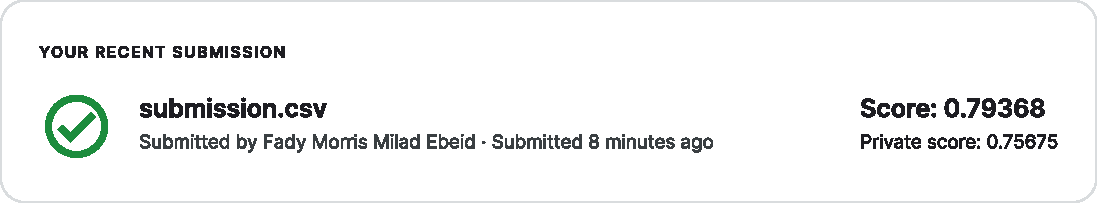
\includegraphics[scale=0.8]{kaggle-test-score}
    \end{figure}


    \pagebreak

    \subsection{Justification}
    \label{sec:justification}
    
    The final results are summarized in \autoref{tab:kaggle-score-comparison} and \autoref{fig:kaggle-score-comparison}. It shows that our final \emph{XGBoost} model has achieved an AUC-ROC score of \textbf{0.79368} for the test dataset on the Kaggle competition, Improving on the benchmark score of \textbf{0.71541} by $\approx 11\%$. 

    \begin{table}[H]
      \centering
      \caption{Comparison Between the Benchmark Model and the Final Model's AUC-ROC score}
      \label{tab:kaggle-score-comparison}
      \begin{tabular}{llr}
        \toprule
        Model & private score & public score \\
        \midrule
        Benchmark(Logistic Regression) & 0.71265 & 0.71541 \\
        XGBoost Model  & 0.75675 & 0.79368 \\
        \bottomrule
      \end{tabular}
    \end{table}

    \begin{figure}[H]
      \centering
      \caption{A Comparison Between Benchmark Model and Final Model Scores}
      \label{fig:kaggle-score-comparison}
      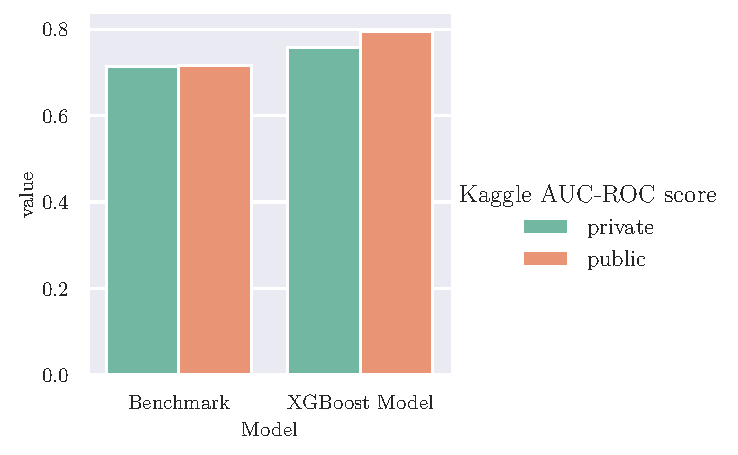
\includegraphics{08_score-comparison}
    \end{figure}


\pagebreak
    \section{Conclusion}
    
    \subsection{Reflection}
    In this project, we used the Arvato dataset to predict whether an individual targeted by the mailout campaign will turn into a client or not.

    The dataset was very challenging to work with, it was highly dimensional with lots of inconsistencies, missing values, and invalid values. For such a dataset, the scikit-learn pipeline and transformers came in handy to develop a robust preprocessing workflow.

    From this project, it was clear that \emph{XGBoost} is one of the top-performing machine learning algorithms. That's why it is used in Kaggle competitions.
    
    The entire end-to-end solution to the problem can be summarized in the following steps:
    \begin{enumerate}
    \item The problem was clearly defined, then the candidate solution algorithms and benchmark metrics were selected according to the nature of the problem.
    \item The training dataset and metadata were checked for problems and inconsistencies in the exploratory data analysis phase.
    \item The metadata was cleaned and saved for use throughout the project. The dataset features were categorized into numerical, ordinal, and nominal.
    \item The training dataset features were examined for mismatch with the metadata. Then we explored missing data, correlated features, duplicate training samples, and outliers.
    \item A preprocessing pipeline was developed using the best software engineering practices of code reuse. We extended scikit-learn transformers and adapted them to the current problem at hand.
    \item The training and the testing dataset were processed using the developed pipeline.
    \item The training dataset was split further into train and validation sets.
    \item A benchmark model was developed, tested on the test data and the metric score was recorded.
    \item The datasets were uploaded to an AWS S3 Bucket to be used by Amazon SageMaker.
    \item A preliminary SageMaker estimator was created to train an \emph{XGBoost} model using an Amazon SageMaker built-in algorithm container image.
    \item The model was further refined using an Amazon SageMaker hyperparameter tuning job to select the best hyperparameters according to the objective metric specified.
    \item A final \emph{XGBoost} model was trained using the best hyperparameters discovered by the tuning job.
    \item The final model was used for inference to generate predictions from the test data again, obtaining a vector of probabilities. Then the results were submitted to Kaggle API to get another metric score.
    \item The final \emph{XGBoost} model was evaluated and compared to the benchmark model. It was clear that the final model outperformed the benchmark model and got higher AUC-ROC scores.
    \end{enumerate}
    
    \subsection{Improvement}
    The results achieved in this project could be possibly improved by the following suggestions:
    \begin{enumerate}
    \item Increasing the hyperparameter tuning job's \code{'max_jobs'} parameter to allow the tuner to run for a longer period and search for a better combination of hyperparameters in the search space.
    \item Trying to use the \href{https://docs.aws.amazon.com/sagemaker/latest/dg/automatic-model-tuning-considerations.html#automatic-model-tuning-log-scales}{logarithmic scales} for some hyperparameters in hyperparameter tuning.
    \item Investigating oversampling techniques (such as SMOTE) and undersampling techniques to address the problem of class imbalance.
    \item A more thorough understanding of the dataset features.
    \item Investigating feature importance and retraining the algorithm using $k$-most important features.
    \item Examining the correlation between categorical nominal variables using the chi-square test.
    \end{enumerate}
    \newpage




    \printbibliography[heading=bibintoc] %print bibliography and add entry to table of contents

    \newlength{\mytextsize}

    % Display current font size
    % \makeatletter
    % \show\f@size
    % \setlength{\mytextsize}{\f@size pt}
    % \makeatother
    % \showthe\mytextsize
    % \makeatother

  \end{document}

  %%% Local Variables:
  %%% mode: latex
  %%% TeX-master: t
  %%% LaTeX-command: "latex -shell-escape"
  %%% End:
